\documentclass[a4paper,12pt]{article}
\usepackage[english]{babel}
\usepackage[utf8]{inputenc}

%
% For alternative styles, see the biblatex manual:
% http://mirrors.ctan.org/macros/latex/contrib/biblatex/doc/biblatex.pdf
%
% The 'verbose' family of styles produces full citations in footnotes, 
% with and a variety of options for ibidem abbreviations.
%
\usepackage{graphicx}
\usepackage{csquotes}
\usepackage[style=verbose-ibid,backend=bibtex]{biblatex}
\bibliography{sample}

\usepackage{lipsum} % for dummy text

\title{Mastering The game of Go without human knowledge}

\author{Shayan Amani}

\date{\today}

\begin{document}
\maketitle

\section{Intro}
Making a Deep-Reinforcement Learning model (namely Alpha Go and later Alpha Go Zero) in order to train an agent to make decisions (basically play the game) in Go game. They have started with extracting a set of policies by observing and training many samples of games and moves played by human top players in Go utilizing a supervised learning method and then fed the policy to a Reinforcement Learning model to evaluate the value function. They have proposed a reduction strategy in terms of breadth and depth of search space tree. Speaking technically, narrowing down the breadth of the tree using policy set and secondly replacing down hand sub-trees with a value from value set. Based on Monte Carlo tree search, firstly it traverses from root to leaf and then selects actions action from value network (Q) and then select actions in favor of policy network (U). Secondly, an expansion is done on leaf nodes with examination on policy and value network. Finally, it backs up to the search tree with maintaining a mean evaluation seen onward from each edges (Q).
 
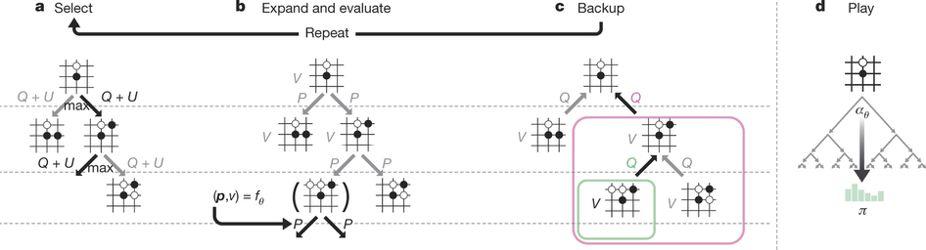
\includegraphics[scale=0.5]{tree.jpg}


\section{Alpha Go Zero}
First of all, all human data has been removed from the plot of the solution just make the agent powerful enough to play with minimum human-assisted helps (data or feature) possible, In other words, building a  pure Reinforcement Learning model. Moreover, They have tried to merge policy and value networks to come up with a single neural network. 

\section{Conclusion}
Showing this huge improvement from the previous version (Alpha Go Sedol) is astounding enough to rely on a self-play model which can start randomly and continue only on it's merely own.
 


% This is an example citation \autocite{ginsberg}.
% \lipsum[1] % dummy text

% This is another example citation \autocite{brassard}.
% \lipsum[2] % dummy text

% This is a repeated citation \autocite{brassard}.
% \lipsum[3] % dummy text

% This is another example citation \autocite{adorf}.
% \lipsum[4] % dummy text 

\end{document}